\documentclass[conference]{IEEEtran}

\usepackage{amssymb,amsmath,epsfig,graphics,enumerate,float,subfigure,verbatim,url,multirow,caption}
\usepackage[usenames,dvipsnames]{color}
\usepackage[vlined,ruled]{algorithm2e}
\usepackage{tikz,alltt,arydshln,longtable,listings,bm}
\usepackage{listings}
\usepackage{caption}
\usepackage{graphicx}
%\usepackage{float}
 
%\newcommand{\comment}[1]{} 
\newcommand{\etc} {\emph{etc.}}
\newcommand{\etal}{\emph{et~al. \/}}
\newcommand{\eg}  {\emph{e.g., \/}}
\newcommand{\ie}  {\emph{i.e., \/}}
\def\Reals{\mathbf{R}}
\def\Ints{\mathbf{Z}}
\def\Nats{\mathbf{N}}
\def\E{\mathbb{E}}
\def\P{\mathbb{P}}
\def\A{{\cal A}}
\def\bf{\bfseries}
\newcommand{\nop}[1]{}
\newcommand{\from}[2]{{\bf [{\sc from #1:} #2]}}
\newcommand{\ra}{\mbox{$\rightarrow\;$}}
\newcommand{\rax}{\mbox{$\;\rightarrow\;$}}
\newcommand{\lb}{\mbox{$\langle$}}
\newcommand{\rb}{\mbox{$\rangle$}}
\newcommand{\cln}{\mbox{$:$}}
\newcommand{\crossdouble}{\makebox[2.85ex]{\bf ---}\makebox[-2.95ex]{}}
\newcommand{\st}{\mbox{$\ast$}}
\def\ssp{\mbox{\hspace*{2.5ex}}}
\def\sp{\mbox{\hspace*{6.5ex}}}
\def\Bsp{\mbox{\hspace*{30ex}}}
\def\dq{\mbox{''}}
\def\cod{\mbox{$~:-~$}}
\def\parag{{\vspace{0.01in} }}
\def\boxend{\hspace*{\fill} $\blacksquare$}
\def\qed{\hspace*{\fill} $\blackbox$}
%\def\QED{\mbox{\rule[0pt]{1.5ex}{1.5ex}}}
\def\proof{\noindent\hspace{2em}{{\itshape Proof: }}}
\def\endproof{\hspace*{\fill}~\qed\par\endtrivlist\unskip}

\begin{document}
\title{Tutorial for Sound Transcription and Piano Score Following\\
\vspace*{-20pt}}

\author{Stephen Moskal\\
%\IEEEauthorblockN{Stephen Moskal}
%Department of Computer Engineering\\
Rochester Institute of Technology, Rochester, New York 14623
}
\maketitle

\begin{abstract}
Detection and transcription of piano keys from just examining frequencies unassisted can be extremely inaccurate even on single notes due to noise in the recordings and the similarities between notes.  This becomes even more troubling when complex chords are played or the tempo is increased to a fast pace.  However if a system is trained to the notes beforehand with either single notes or a score with the use of Support Vector Machines, the accuracy of transription is improved significantly when compared to using just the frequency of the sound as the feature set.  This work proposes to train a system using various features of a recording of a score and be able to identify where in the score is playing at any given time live.  By identifying the section where the player is playing in a score of music, different events in a virtual stage can be triggered on screen like lights, colors, or videos.
\end{abstract}

\section{Introduction}
\label{sec:intro}
For live performances of music, the actual music is the main draw for audiences but also the ambiance, lights, and spectacle of the show plays a major role in the appeal of a live performance.  The days of the underground basement rock band performances are still around however there is an increasing demand for performers to have their shows stand out in someway.  Whether it is The Flaming Lips with hundreds of balloons, confetti, and gloves with high powered lasers or U2 with massive transforming stages hundreds of feet high, it all adds to the experience.  The goal of this work is to create a framework in which performers can input their music into a system and be able to control certain aspects of their show depending on what music they are playing.  Most live shows will use some sort of sound based system to trigger lights, pyrotechnics, or videos.  However these systems are based on either the elapsed time from the beginning of the song the performance is in, or just a large change in volume.  This work instead trains a system before hand to the music and classifies sections of the music meaning that different events can be triggered when a specific note is played.

There are benefits to a system like this as it allows for plenty of flexibility of how a performance can be structured.  By a note based classification system, the performer does not need a technician to start and stop the system in between songs since the time in between songs varies.  The performer could be communicating with the audience, taking a drink, or changing their instrument, meanwhile the system is listening for the note that starts the next song.  Once that specific note is played, the show automatically begins with no interaction after the system is trained to the set.  The scope of this work focuses on piano pieces where the training set is a recording of the song and the system will listen live looking for sections of the recording.  However although this paper specifically uses the piano, it can be trained to any instrument including voices or other sounds.

\section{System Requirements}
\label{sec:arch}
The purpose of this work is to have a simple requirements that allows for portability of code and minimal hardware to use fully.  The programming language Python 2.7 was chosen due to its widespread use, portability, and a massive open source library support.  As for hardware, the only requirements is a microphone connected to the machine running the software.  The test machine used in this work is a 2013 Macbook Pro using the internal microphone, however other devices like a Raspberry Pi with an external microphone can be used if a more specialized device is desired.   All libraries used in this work are open source and freely available.

To begin, three libraries need to be installed for audio streaming, feature extraction, and classification.  First is PyAudio which handles all of the interfacing between the program and the microphone.  PyAudio can be configured to use any microphone on the system along with reading in sound files from outside of the program.  Another benefit of PyAudio is that it allows for multi-threading which will be crucial later on for live streaming of data.  Next is the package Aubio which handles taking the data from the file and applying Fast Fourier Transforms and then feature extraction off of the transform.  Aubio provides API's that can automatically apply filters to the incoming sounds and organize data for classification.  Then lastly, the package Scikit-Learn is used to handle all of the machine learning and classification of the data.  Sklearn is an extremely powerful package that allows for supervised training techniques like Classifcation Trees, Support Vector Machines , etc. along with unsupervised learning techniques like Neural Networks and clustering.  

\section{Implementation}
\label{sec:impl}

The input of the program is a waveform file (wav) which will act as the training set for the program.  The program starts with reading in the sound file and then from there extracting features from the file.  Then the data is cleaned up as there are many unwanted features.  These features are then assigned a class depending on the frequency of the tone which is used for the classification of the times.  Using SKLearn, the test data is then classified using a Support Vector Machine.  Once classified, the program then listens in through the microphone in a multi-threaded structure.  

\subsection{Program Constants}
\label{sec:const}

To optimize the running of the program and the classification of the notes there are some tune-able parameters for various functions.  For optimizing the program for pitch detection, the window in which the FFT is performed on if can be adjusted if desired.  Then when the pitch is calculated the confidence of the value is reported and a parameter can be set to throw out some values if desired.  The current tolerance by default is to only accept values with a confidence of .9 or higher.  A higher or lower value should be changed depending on the aggressiveness of the data fit desired.  When the data is assigned to the classes, there is a small tolerance in Hz that will define a window in which classes are similar.  If there are the same note played in the training set multiple times, it will assign those to the same class instead of separate.  Lastly, to finely tune the program to a specific range in the spectrum (in this case a piano) constants can be tuned to restrict the classification to just the possible spectrum of the instrument.  In the case of a standard piano, it is set to 30Hz for 5000Hz.

\subsection{Feature Selection}
\label{sec:feat}
Picking the feature set is the most important aspect to get correct for accurate classification.  Using Aubio, feature extraction is quite simple.  For each window, the FFT of the signal is taken and different functions from Aubio are used to extract features automatically.  The first feature to extract is what is called the onset, which is the start a note.  This is done by taking the sample and calling the onset method on the Audio onset object.  As seen below in Figure 1, the onset is shown as a vertical line where the raw waveform is the top graph and the amplitude is on the bottom.

\begin{figure}[htb]
\centering 
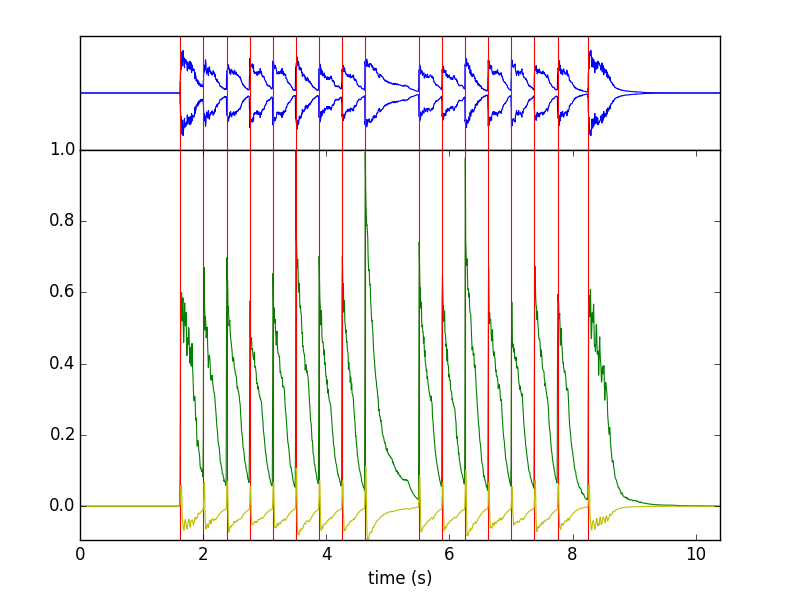
\includegraphics[width=.48\textwidth]{onsets.png}
\caption{A graph showing the onsets of each note of a song.}
\vspace*{-20pt}
\label{fig:onset}
\end{figure}

Next for assigning the classes to the data, the pitches of each of the sample are calculated using Aubio again. Using the pitch function with in Aubio, both the estimated pitch and also the confidence of the correctness of the pitch.  With the input of the program being a simple scale, Figure 2 below shows the pitch in Hertz and it's corresponding confidence level for the sample.  Classes can be assigned by looking at the frequency in between each onset and assigning a class for similar frequencies.

\begin{figure}[htb]
\centering 
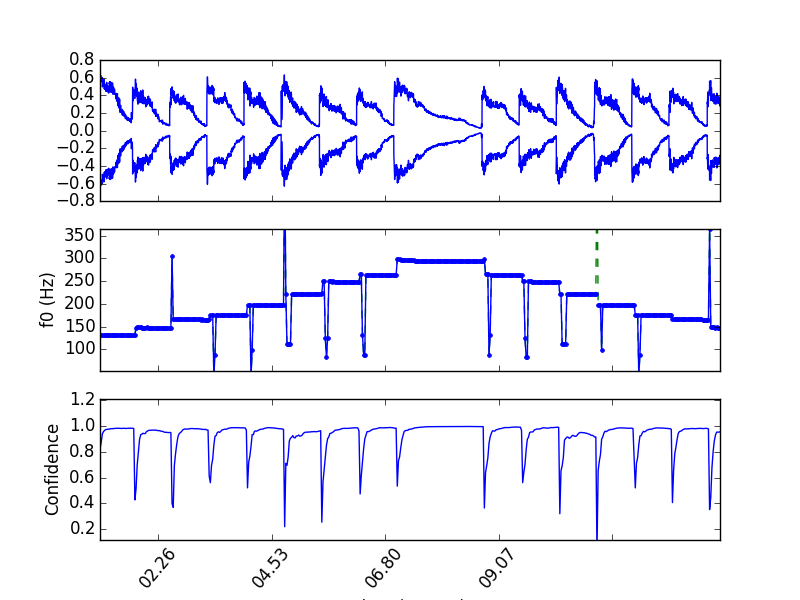
\includegraphics[width=.48\textwidth]{pitch.png}
\caption{A graph showing pitches of the sound file over time.}
\vspace*{-20pt}
\label{fig:pitch}
\end{figure}

Because the frequencies of the samples varies so much even in the same section of the note, stronger features that still describe the sounds are desired.  To do this, the energy at 40 separate bands of the frequency bands are taken over time.  This will allow for very accurate classification since even though frequencies of the notes and chords may be very close together, the different parts of the spectrum that note may excite could be very different.  This allows for notes to be very separable from each other instead of simply just using the frequency of the transcribed notes.  Figure 3 below shows same data set as before but also showing the energy for 40 different bands of the spectrum.

\begin{figure}[htb]
\centering 
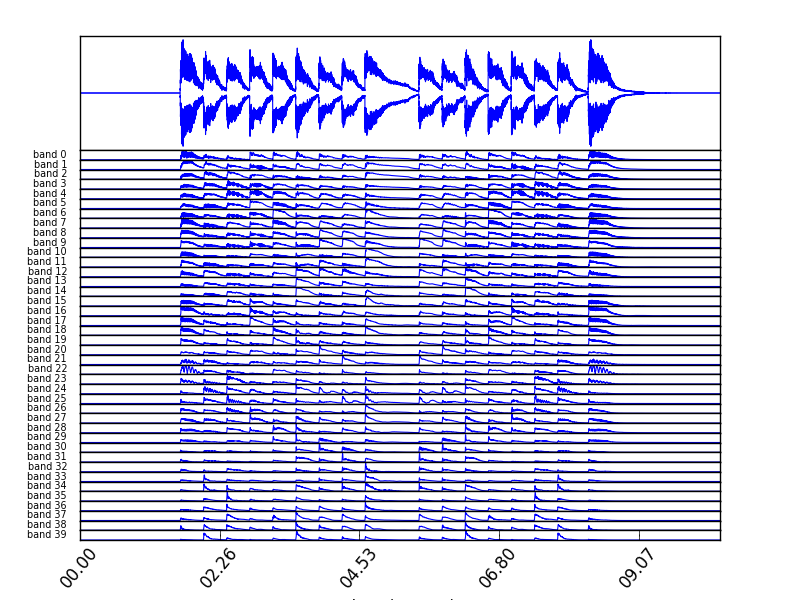
\includegraphics[width=.48\textwidth]{energy.png}
\caption{A graph showing the sound energy for 40 bands in the audio spectrum.}
\vspace*{-20pt}
\label{fig:energy}
\end{figure}

Notice that even though the notes on the piano are close together, the overall energy across the bands are very different.  However for the same note the energies are similar to each other meaning that this is a good feature to describe the data.  In this work this is the features that will be used for classification but they will need to be organized properly to be used in the classifier.

\subsection{Data Organization}
\label{sec:org}

The classifiers in SKLearn require the data to be organized in a fashion where the data used for the X dimensions are separated from the data in the Y dimension.  The X data array describes the features that were extracted from before.  In this case the features will be the frequencies and the energies of the sounds.   However the data Y, which is the class that the corresponding X data belongs to, needs to be set in a supervised fashion.  To do this, the onsets of each of the notes are used.  It can be assumed that the samples in between each onset are going to belong to the same class since they are all one note.  However there may be similar notes in the set that may be played and those should be assigned to the same class which will reinforce the training.   To accomplish this, the average frequency between each onset is found, if some of the samples are below the confidence threshold or outside of the bounds of the set frequency band.  Each of these average values between onsets are assigned a unique class and then assigned to the individual samples.  If one of the average values are close to another average value (with in the set window) they are set to the same class.  Once all the samples are assigned to a class, the Y data array is created.  Now both of the arrays are created and then can be inserted into the classifier.  

\subsection{Classification}
\label{sec:class}

The SKLearn package makes the feat of classification extremely trivial once the type of classification chosen and the data is organized correctly.  This work uses the classification technique of Support Vector Machine due to a relatively low amount of data per class but a high amount of features.  The robustness of the SVM as compared to a more primitive classification technique like Classification Trees benefits the accuracy and the speed of the system while not providing anymore complexity from a coding perspective.  To use the SVM, a simple initialization call of to the SVM import object, svm.SVC(), which returns a classifier object.  Then the data is sent into this classifier object to create the model using the method clf.fit(Xdata, Ydata).  Then to make a prediction the predict function in the same classifier object, clf.predict(Xtest), is used with the testing X value.  This will return the class in which it predicts that the input belongs to, making it extremely easy to classify and make predictions. 

\subsection{Audio Streaming}
\label{sec:stream}
The last section of the code is the part that handles listening from the microphone live and then making predictions of the note from the stream.  PyAudio is used to interface with the microphone and then read in chunks of data.  A multi-threaded approach is needed here data needs to be processed on the incoming audio without interrupting the reading in of the audio stream.  Thus, there are two threads running simultaneously in this section of the code.  One is constantly reading audio from the microphone and appending this data into the back of an array.  While another thread is popping data off the top of this array to process and make predictions on the data.  This allows for a uninterrupted data stream and processing happening at the same time.  

On the side that is popping the data off of the array after it has already been read in from the microphone, the feature extraction is done in the same way except slightly out of order.  First, the data is only popped if the array has some thing in it, meaning that it will not process data if it gets ahead of the stream.  Then feature extraction only begins when there is an onset detected.  If there is an onset it will extract the features exactly before and organize them into an X test array.  Then this Xtest array is put into the classifier using the predict method and the class is reported back to the user.

\section{Results}
\label{sec:results}

TODO:  I have do some tweaking to see if I can make it better.

\section{Upcoming Improvements}
\label{sec:improv}

\section{Conclusion}
\label{sec:concl}

TODO: Once the results are sorted out.

\bibliographystyle{IEEETran}
\bibliography{ref}

\end{document}
